En este módulo se incluyen todos los pasos necesarios para el etiquetado de los datos adquiridos con el modelo BERT, su revisión y reetiquetado. El mismo contiene las siguientes secciones:

Etiquetado de Comentarios

La carpeta etiquetadodatos almacena los siguientes archivos:

\begin{itemize}

\item operacion\_dataset.py: Este archivo se encarga de diversas operaciones necesarias para el entrenamiento del modelo BERT, como la mezcla de datos, el conteo de clases y la división de conjuntos de datos. Para más detalles, consulte la figura \ref{fig:uml5}.

\begin{figure}
	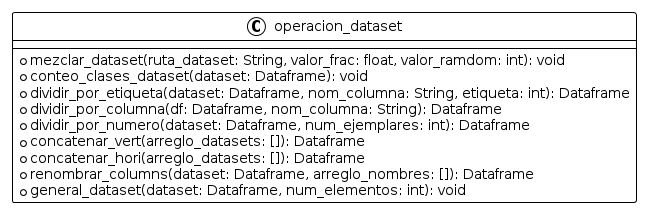
\includegraphics[width=0.65\textwidth]{capitulo5/figuras/fig5.png}
	\caption{Clase operacion\_dataset}
	\floatfoot{Fuente: Elaboración propia, generado con PlantUML}
	\label{fig:uml5}
\end{figure}

\item bert\_multi.py: Este archivo se ocupa de la creación, configuración, entrenamiento y predicción, entre otras tareas específicas del modelo BERT. Para más detalles, consulte la figura \ref{fig:uml6}.

\begin{figure}
	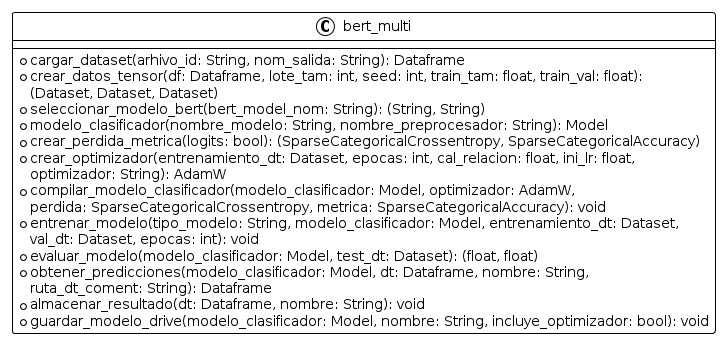
\includegraphics[width=0.65\textwidth]{capitulo5/figuras/fig6.png}
	\caption{Clase bert\_multi}
	\floatfoot{Fuente: Elaboración propia, generado con PlantUML}
	\label{fig:uml6}
\end{figure}

\end{itemize}

Reetiquetado y Revisión de Etiquetas

Para el reetiquetado de los conjuntos de datos, se utilizó la herramienta Label Studio, que acepta archivos en varios formatos como CSV y TSV. Esta herramienta proporciona una interfaz cómoda que agiliza el proceso de revisión, etiquetado y reetiquetado. Además, ofrece filtros y otras funciones que permiten realizar cambios en cualquier conjunto de datos, los cuales pueden exportarse en distintos formatos.


